 %% History:
% Pavel Tvrdik (26.12.2004)
%  + initial version for PhD Report
%
% Daniel Sykora (27.01.2005)
%
% Michal Valenta (3.12.2008)
% rada zmen ve formatovani (diky M. Duškovi, J. Holubovi a J. Žďárkovi)
% sjednoceni zdrojoveho kodu pro anglickou, ceskou, bakalarskou a diplomovou praci

% One-page layout: (proof-)reading on display
%%%% \documentclass[11pt,oneside,a4paper]{book}
% Two-page layout: final printing
\documentclass[11pt,twoside,a4paper]{book}   
%=-=-=-=-=-=-=-=-=-=-=-=--=%
% The user of this template may find useful to have an alternative to these 
% officially suggested packages:
\usepackage[czech, english]{babel}
\usepackage[T1]{fontenc} % pouzije EC fonty 
% pripadne pisete-li cesky, pak lze zkusit take:
% \usepackage[OT1]{fontenc} 
\usepackage[utf8]{inputenc}
%=-=-=-=-=-=-=-=-=-=-=-=--=%
% In case of problems with PDF fonts, one may try to uncomment this line:
%\usepackage{lmodern}
%=-=-=-=-=-=-=-=-=-=-=-=--=%
%=-=-=-=-=-=-=-=-=-=-=-=--=%
% Depending on your particular TeX distribution and version of conversion tools 
% (dvips/dvipdf/ps2pdf), some (advanced | desperate) users may prefer to use 
% different settings.
% Please uncomment the following style and use your CSLaTeX (cslatex/pdfcslatex) 
% to process your work. Note however, this file is in UTF-8 and a conversion to 
% your native encoding may be required. Some settings below depend on babel 
% macros and should also be modified. See \selectlanguage \iflanguage.
%\usepackage{czech}  %%%%%\usepackage[T1]{czech} %%%%[IL2] [T1] [OT1]
%=-=-=-=-=-=-=-=-=-=-=-=--=%

%%%%%%%%%%%%%%%%%%%%%%%%%%%%%%%%%%%%%%%
% Styles required in your work follow %
%%%%%%%%%%%%%%%%%%%%%%%%%%%%%%%%%%%%%%%
\usepackage{graphicx}
%\usepackage{indentfirst} %1. odstavec jako v cestine.

\usepackage{k336_thesis_macros} % specialni makra pro formatovani DP a BP
 % muzete si vytvorit i sva vlastni v souboru k336_thesis_macros.sty
 % najdete  radu jednoduchych definic, ktere zde ani nejsou pouzity
 % napriklad: 
 % \newcommand{\bfig}{\begin{figure}\begin{center}}
 % \newcommand{\efig}{\end{center}\end{figure}}
 % umoznuje pouzit prikaz \bfig namisto \begin{figure}\begin{center} atd.


%%%%%%%%%%%%%%%%%%%%%%%%%%%%%%%%%%%%%
% Zvolte jednu z moznosti 
% Choose one of the following options
%%%%%%%%%%%%%%%%%%%%%%%%%%%%%%%%%%%%%
%\newcommand\TypeOfWork{Diplomová práce} \typeout{Diplomova prace}
% \newcommand\TypeOfWork{Master's Thesis}   \typeout{Master's Thesis} 
\newcommand\TypeOfWork{Bakalářská práce}  \typeout{Bakalarska prace}
% \newcommand\TypeOfWork{Bachelor's Project}  \typeout{Bachelor's Project}


%%%%%%%%%%%%%%%%%%%%%%%%%%%%%%%%%%%%%
% Zvolte jednu z moznosti 
% Choose one of the following options
%%%%%%%%%%%%%%%%%%%%%%%%%%%%%%%%%%%%%
% nabidky jsou z: http://www.fel.cvut.cz/cz/education/bk/prehled.html

%\newcommand\StudProgram{Elektrotechnika a informatika, dobíhající, Bakalářský}
%\newcommand\StudProgram{Elektrotechnika a informatika, dobíhající, Magisterský}
% \newcommand\StudProgram{Elektrotechnika a informatika, strukturovaný, Bakalářský}
% \newcommand\StudProgram{Elektrotechnika a informatika, strukturovaný, Navazující magisterský}
\newcommand\StudProgram{Softwarové technologie a management, Bakalářský}
% English study:
% \newcommand\StudProgram{Electrical Engineering and Information Technology}  % bachelor programe
% \newcommand\StudProgram{Electrical Engineering and Information Technology}  %master program


%%%%%%%%%%%%%%%%%%%%%%%%%%%%%%%%%%%%%
% Zvolte jednu z moznosti 
% Choose one of the following options
%%%%%%%%%%%%%%%%%%%%%%%%%%%%%%%%%%%%%
% nabidky jsou z: http://www.fel.cvut.cz/cz/education/bk/prehled.html

%\newcommand\StudBranch{Výpočetní technika}   % pro program EaI bak. (dobihajici i strukt.)
%\newcommand\StudBranch{Výpočetní technika}   % pro prgoram EaI mag. (dobihajici i strukt.)
\newcommand\StudBranch{Softwarové inženýrství}            %pro STM
%\newcommand\StudBranch{Web a multimedia}                  % pro STM
%\newcommand\StudBranch{Computer Engineering}              % bachelor programe
%\newcommand\StudBranch{Computer Science and Engineering}  % master programe


%%%%%%%%%%%%%%%%%%%%%%%%%%%%%%%%%%%%%%%%%%%%
% Vyplnte nazev prace, autora a vedouciho
% Set up Work Title, Author and Supervisor
%%%%%%%%%%%%%%%%%%%%%%%%%%%%%%%%%%%%%%%%%%%%

\newcommand\WorkTitle{Ruby - Access Control List}
\newcommand\FirstandFamilyName{Jan Širl}
\newcommand\Supervisor{Ing. Pavel Strnad}


% Pouzijete-li pdflatex, tak je prijemne, kdyz bude mit vase prace
% funkcni odkazy i v pdf formatu
\usepackage[
pdftitle={\WorkTitle},
pdfauthor={\FirstandFamilyName},
bookmarks=true,
colorlinks=true,
breaklinks=true,
urlcolor=red,
citecolor=blue,
linkcolor=blue,
unicode=true,
]
{hyperref}



% Extension posted by Petr Dlouhy in order for better sources reference (\cite{} command) especially in Czech.
% April 2010
% See comment over \thebibliography command for details.

\usepackage[square, numbers]{natbib}             % sazba pouzite literatury
%\usepackage{url}
%\DeclareUrlCommand\url{\def\UrlLeft{<}\def\UrlRight{>}\urlstyle{tt}}  %rm/sf/tt
%\renewcommand{\emph}[1]{\textsl{#1}}    % melo by byt kurziva nebo sklonene,
\let\oldUrl\url
\renewcommand\url[1]{<\texttt{\oldUrl{#1}}>}




\begin{document}

%%%%%%%%%%%%%%%%%%%%%%%%%%%%%%%%%%%%%
% Zvolte jednu z moznosti 
% Choose one of the following options
%%%%%%%%%%%%%%%%%%%%%%%%%%%%%%%%%%%%%
\selectlanguage{czech}
%\selectlanguage{english} 

% prikaz \typeout vypise vyse uvedena nastaveni v prikazovem okne
% pro pohodlne ladeni prace


\iflanguage{czech}{
	 \typeout{************************************************}
	 \typeout{Zvoleny jazyk: cestina}
	 \typeout{Typ prace: \TypeOfWork}
	 \typeout{Studijni program: \StudProgram}
	 \typeout{Obor: \StudBranch}
	 \typeout{Jmeno: \FirstandFamilyName}
	 \typeout{Nazev prace: \WorkTitle}
	 \typeout{Vedouci prace: \Supervisor}
	 \typeout{***************************************************}
	 \newcommand\Department{Katedra počítačů}
	 \newcommand\Faculty{Fakulta elektrotechnická}
	 \newcommand\University{České vysoké učení technické v Praze}
	 \newcommand\labelSupervisor{Vedoucí práce}
	 \newcommand\labelStudProgram{Studijní program}
	 \newcommand\labelStudBranch{Obor}
}{
	 \typeout{************************************************}
	 \typeout{Language: english}
	 \typeout{Type of Work: \TypeOfWork}
	 \typeout{Study Program: \StudProgram}
	 \typeout{Study Branch: \StudBranch}
	 \typeout{Author: \FirstandFamilyName}
	 \typeout{Title: \WorkTitle}
	 \typeout{Supervisor: \Supervisor}
	 \typeout{***************************************************}
	 \newcommand\Department{Department of Computer Science and Engineering}
	 \newcommand\Faculty{Faculty of Electrical Engineering}
	 \newcommand\University{Czech Technical University in Prague}
	 \newcommand\labelSupervisor{Supervisor}
	 \newcommand\labelStudProgram{Study Programme} 
	 \newcommand\labelStudBranch{Field of Study}
}




%%%%%%%%%%%%%%%%%%%%%%%%%%    Poznamky ke kompletaci prace
% Nasledujici pasaz uzavrenou v {} ve sve praci samozrejme 
% zakomentujte nebo odstrante. 
% Ve vysledne svazane praci bude nahrazena skutecnym 
% oficialnim zadanim vasi prace.
{
\pagenumbering{roman} \cleardoublepage \thispagestyle{empty}
\chapter*{Na tomto místě bude oficiální zadání vaší práce}
\begin{itemize}
\item Toto zadání je podepsané děkanem a vedoucím katedry,
\item musíte si ho vyzvednout na studiijním oddělení Katedry počítačů na Karlově náměstí,
\item v jedné odevzdané práci bude originál tohoto zadání (originál zůstává po obhajobě na katedře),
\item ve druhé bude na stejném místě neověřená kopie tohoto dokumentu (tato se vám vrátí po obhajobě).
\end{itemize}
\newpage
}

%%%%%%%%%%%%%%%%%%%%%%%%%%    Titulni stranka / Title page 

\coverpagestarts

%%%%%%%%%%%%%%%%%%%%%%%%%%%    Podekovani / Acknowledgements 

\acknowledgements
\noindent
Chtěl bych především poděkovat panu Ing. Pavlu Strnadovi%, že se mě ujal jako vedoucí prácí a poskytl mi rady motivaci. Poděkování také patří mé přítelkyni a rodině za nemalou podporu při tvorbě bakalářské práce a v průběhu celého studia.

%%%%%%%%%%%%%%%%%%%%%%%%%%%   Prohlaseni / Declaration 

\declaration{V~Praze dne 25.\,5.\,2012}
%\declaration{In Prague on March 18, 2012}


%%%%%%%%%%%%%%%%%%%%%%%%%%%%    Abstract 
 
\abstractpage

This paper presents the design and implementation of library management access rights in the programming language Ruby.

The library is designed for object database CellStore and is solved using the Access Control List. Library used for storing and querying the database itself, which communicates with the protocol XML-RPC (Remote Procedure Call) XQuery and XQuery Update Facility.
The functionality of the library was developed and tested on eXistDB.

% Prace v cestine musi krome abstraktu v anglictine obsahovat i
% abstrakt v cestine.
\vglue60mm

\noindent{\Huge \textbf{Abstrakt}}
\vskip 2.75\baselineskip

\noindent
Tato práce prezentuje návrh a realizaci knihovny pro správu přístupových práv v programovacím jazyku Ruby. 

Knihovna  je určena pro objektovou databázi Cellstore a je řešena pomocí Access Control List. Knihovna využívá pro ukládání a dotazování samotnou databázi, se kterou komunikuje pomocí protokolu XML-RPC (Remote Procedure Call) technologií xQuery a xQuery Update Facility. 
Funkčnost knihovny byla vyvíjena a testována na eXistDB.


\noindent
%Očekávají se cca 1 -- 2 odstavce, maximálně půl stránky.

%%%%%%%%%%%%%%%%%%%%%%%%%%%%%%%%  Obsah / Table of Contents 

\tableofcontents


%%%%%%%%%%%%%%%%%%%%%%%%%%%%%%%  Seznam obrazku / List of Figures 

\listoffigures


%%%%%%%%%%%%%%%%%%%%%%%%%%%%%%%  Seznam tabulek / List of Tables

\listoftables


%**************************************************************

\mainbodystarts
% horizontalní mezera mezi dvema odstavci
%\parskip=5pt
%11.12.2008 parskip + tolerance
\normalfont
\parskip=0.2\baselineskip plus 0.2\baselineskip minus 0.1\baselineskip

% Odsazeni prvniho radku odstavce resi class book (neaplikuje se na prvni 
% odstavce kapitol, sekci, podsekci atd.) Viz usepackage{indentfirst}.
% Chcete-li selektivne zamezit odsazeni 1. radku nektereho odstavce,
% pouzijte prikaz \noindent.

%**************************************************************

% Pro snadnejsi praci s vetsimi texty je rozumne tyto rozdelit
% do samostatnych souboru nejlepe dle kapitol a tyto potom vkladat
% pomoci prikazu \include{jmeno_souboru.tex} nebo \include{jmeno_souboru}.
% Napr.:
% \chapter{Úvod}

\section{Úvod do problematiky}

Tato bakalářská práce navazuje na můj semestrální projekt. Zabývá se správou - administrací řízení přístupu, jakožto procesu autorizování uživatelů, skupin a počítačů pro přístup k objektům. Tento proces pracuje s pojmy: oprávnění, uživatelská práva a audit objektů. Tato jednotlivá přiřazená oprávnění začleňuje jako položky řízení přístupu (ACE\footnote{Access Control Entry}) a jejich celé sady začleňuje do seznamu přístupových práv (ACL\footnote{Access Control List}). Úkolem bakalářské práce bylo vytvořit, navrhnout a realizovat v jazyce Ruby model uživatelských přístupových práv určený pro objektovou XML\footnote{Extensible Markup Language} databázi.

Součástí práce byl návrh knihovny. Navržená knihovna realizuje správu řízení přístupu pomocí ACL. Knihovnu nazývám Ruby-ACL. Protože moje bakalářská práce je prací implementační, včetně testů navržené knihovny, zaměřil jsem se na specifikaci rozhraní knihovny a na příklady jejího použití. Výsledkem je nejen samotná realizace knihovny, ale i podrobná programátorská dokumentace.

Je-li potřeba zabezpečit zdroje a jeho prostředky, je nutné vzít v úvahu, jakými právy budou disponovat ti, kteří k nim budou přistupovat. Zabezpečit objekt, například dokument či kolekci, lze přidělením oprávnění, která umožňují uživatelům nebo skupinám provádět u tohoto objektu určité akce. Řízení přístupů je činnost zabývající se přidáváním a zamítáním oprávnění přistupujícím.

Ruby je objektově orientovaný, interpretovaný skriptovací programovací jazyk. Díky své jednoduché syntaxi je poměrně snadný, přesto však dostatečně výkonný, aby dokázal konkurovat známějším jazykům jako je Python a Perl. Převzato a upraveno z wikipedie\cite{wiki:Ruby}

ACL je seznam pro řízení přístupů. Seznam určuje, kdo nebo co má povolení přistupovat k objektu a jaké operace s ním může nebo nesmí provádět. V typickém ACL specifikuje každý záznam v seznamu uživatele a operaci\cite{wiki:acl}.

%-------------------------------

\section{Motivace}
Zaujala mě problematika práv, databází a pro mě neznámého jazyka Ruby.
Jádro celé mé motivace, bylo projít si vývojem softwaru, v tomto případě knihovny, od návrhu přes implementaci k testování a dokumentaci a ověřit si získané poznatky z předmětu softwarového inženýrství. Soustředil jsem se na vlastní nápady. Nechtěl jsem skládat a kopírovat polotvary a "lepit" je dohromady.
% \include{2_teorie}

% atd...

%*****************************************************************************
\chapter{Úvod}

\section{Úvod do problematiky}
Řízení uživatelských práv...

Ruby je programovací jazyk ...

ACL je zkratka pro access control list...

Cellstore je XML databáze ...


Tato bakalářská práce navazuje na můj semestrální projekt. Jejím úkolem bylo vytvořit, navrhnout a realizovat v jazyce Ruby model uživatelských přístupových práv určenou pro objektovou databázi Cellstore. V současnosti neexistuje žádný model uživatelských přístupových práv pro Cellstore. 

Součástí práce byl návrh knihovny. Navržený modul realizuje správu řízení přístupu pomocí ACL (Access Control List). Protože moje bakalářská práce je prací implementační, včetně testů navrženého modulu, zaměřil jsem se na specifikaci rozhraní knihovny a na příklady jejího použití.

Výsledkem bakalářské práce je nejen samotná realizace knihovny, ale i podrobná programátorská dokumentace.

\section{Motivace}



%*****************************************************************************
\chapter{Popis problému, specifikace cíle}

\begin{itemize}
\item Popis řešeného problému, vymezení cílů DP/BP a požadavků na implementovaný systém.
\item Popis struktury DP/BP ve vztahu k vytyčeným cílům.
\item Rešeršní zpracování existujících implementací, pokud jsou známy.
\end{itemize}

\section{Popis řešeného problému}

XML databáze Cellstore v současné době nemá žádný model uživatelských přístupových práv. Bylo potřeba tento nedostatek vyřešit knihovnou implementovanou v jazyce Ruby, protože v Ruby je něco napsané asi engine DB aplikace nebo samotna DB. Mnou naimplementovaná knihovna Ruby ACL řeší problém se spravováním přístupových práv.

\section{Vymezení cílů a požadavků}
Cílem bakalářská práce bylo navrhnout, realizovat a otestovat knihovnu v jazyce Ruby, která bude spravovat uživatelská přístupová práva pro objektovou databázi Cellstore.
Vytyčil jsem si vytvořit co nejjednodušší knihovnu, která by splňovala všechna kritéria zadání. Nechtěl jsem jsem používat a "lepit" dohromady existující moduly a knihovny, které danou problematiku řeší, protože jsem chtěl vytvořit něco svého a projít si vývojem softwaru od požadavků přes analýzu a návrh k realizaci a testování. 
I když Ruby ACL je primárně určena pro XML databázi Cellstore chtěl jsem, aby byla použitelná i pro jiné databáze a reálné přístupy do budov apod.
Určil jsem si, že by bylo pěkné, kdyby knihovna umožňovala jemně nastavit přístupy (Tzv.„fine-grained“).

Seznam požadavků je popsán v tabulce 2.1.
K určení operace a objektu z dotazu bude použit SQL parser třetí strany.

\section{Popis struktury bakalářské práce ve vztahu k vytyčeným cílům}

V analýze je analýza.
V realizaci je realizace.
V testování je testování.

\begin{table}%[h]
\begin{center}
\begin{tabular}{|l|p{9cm}|l|}
\hline
\textbf{id} & \textbf{Specifikace požadavků na software} & \textbf{priorita} \\
\hline
\multicolumn{3}{|l|}{FUNKČNÍ POŽADAVKY} \\
\hline
0 & Ruby ACL je knihovna v jazyce Ruby. Ruby bude umožňovat řízení přístupů pomocí ACL & povinný\\
\hline
1.0 & Ruby ACL bude umožňovat definovat zmocnitele (principals) & povinný\\
\hline
1.1 & Ruby ACL bude umožňovat definovat oprávnění (privileges) & povinný\\
\hline
1.2 & Ruby ACL bude umožňovat definovat  zdrojové objekty (resource objects) & povinný\\
\hline
1.3 & Ruby ACL bude umožňovat editovat or mazat zmocnitele (principals) & povinný\\
\hline
1.4 & Ruby ACL bude umožňovat editovat or mazat oprávnění (privileges) & povinný\\
\hline
1.5 & Ruby ACLbude umožňovat editovat or mazat zdrojové objekty (resource objects) & povinný\\
\hline
1.6 & Ruby ACL bude umožňovat definovat, editovat a mazat pravidla přístupu (ACE) & povinný\\
\hline
2.0 & Ruby ACL bude umožňovat vytvářet ACL & povinný\\
\hline
2.1 & Ruby ACL bude umožňovat načítat a ukládat ACL z a do XML souboru & povinný\\
\hline
2.2 & XML soubor bude definovaný pomocí DTD or XML Schema & povinný\\
\hline
2.3 & XML soubor bude "well formated" podle W3C doporučení & povinný\\
\hline
3.0 & Ruby ACL will offer Default-Deny policy (At the beginning nobody cannot access to anywhere) or Default-Allow policy (At the beginning everybody can access to everywhere) & povinný\\
\hline
4.0 & Ruby ACL bude používat XML-RPC rozhraní ke komunikaci s databází & povinný\\
\hline
5.0 & Ruby ACL bude testována na eXist DB & povinný\\
\hline
\multicolumn{3}{|l|}{NEFUNKČNÍ POŽADAVKY} \\
\hline
1.0 & Ruby ACL bude naprogramována v jazyce Ruby & povinný \\
\hline
2.0 & Ruby ACL bude vydaná jako RubyGem & volitelný\\
\hline
3.0 & Ruby ACL potřebuje databázi s XML-RPC rozhraním & povinný\\
\hline
4.0 & Ruby ACL potřebuje databázi s podporou xQuery a xQuery Update Facility & povinný\\
\hline
\end{tabular}
\end{center}
\caption{Tabulka funkčních a nefunkčních požadavků. priorita = (povinný, volitelný, nepovinný)}
\label{tab:tab1}
\end{table}

\section{Dostupné knihovny}

Ruby knihovny (lehce je popsat): acl9, activeacl, ... 

Reseni Oracle, phpGACL, Obecne. Take lehce popsat. Hlavni popsani bude v analyze.



%*****************************************************************************
\chapter{Analýza a návrh řešení}
Analýza a návrh implementace (včetně diskuse různých alternativ a volby implementačního prostředí).
Tato kapitola se dělí na analýzu a návrh. V analýze se zaměřilo na prostudování tří existujících řešení. Z informací získaných z dokumentace jsem sestavil návrh pro Ruby ACL.

\section{Analýza}

... proc pomoci acl, popisuje nejznámější rešení acl, 



\subsection{Exitující řešení}

Při řešení vlastního návrhu na model uživatelských přístupových práv jsem vycházel ze dvou zdrojů – známých řešení a jednoho obecného řešení.

\subsubsection{Obecné řešení}
Obecným řešením je držet si tabulku, kde ve sloupcích budou objekty, ke kterým je možno přistupovat a v řádcích jsou přistupující. V poli pak jsou hodnoty boolean, které vyjadřují buď allow nebo deny. Příklad tabulkového řešení je v tabulce 2.1.

\begin{table}%[h]
\centering
%% Some packages, such as MDW tools, offer better commands for making tables
%% than the plain LaTeX2e tabular which is used here.
\begin{tabular}{|r||c|c|c|}
\hline
Who / Where & Surgeryroom & ambulance & Patient's room\\
\hline\hline
Doctors & 1 & 1 & 1\\
\hline
Nurses & X & 1 & 1\\
\hline
Patients & X & X & 1\\
\hline
\end{tabular}
\caption{Obecné řešení modelu práv pomocí matice}
\end{table}

%-------------------------------------

\subsubsection{Oracle}
Jedním z řešení je podnikové řešení prezentované v Oracle® XML DB Developer's Guide, 11g Release 1 (11.1), Part Number B28369-04 na \url{http://docs.oracle.com/cd/B28359_01/appdev.111/b28369/xdb21sec.htm}. Ve stati Access Control Lists and Security Classes je popsán koncept firmy ORACLE.
 
Text popisuje několik podmínek a pojetí řízení přístupu. Každá z popsaných entit, uživatel, role, privilegia, bezpečnostní třídy, Access Control List (ACL) a Access Control Entry (ACE), je realizována deklarativně jako XML dokument nebo fragment.  

Bezpečnostní autorizace vyžaduje definovat, kteří uživatelé, aplikace nebo funkce mohou mít přístup k jakým datům nebo jaké druhy operací mohou provádět. Existují tedy tři dimenze: (1) kteří uživatelé mohou, (2) vykonávat jaké činnosti, (3) na jakých datech. V souvislosti s každou jednotlivou dimenzí hovoříme o (1) principals - zmocnitelích, (2) privileges - oprávněných, a (3) objektech, které korespondují s těmito třemi dimenzemi. Principals mohou být uživatelé nebo role/skupiny.

Principals a privileges (dimenze 1 a 2) jsou deklarativním způsobem spojeni v definovaných seznamech řízení přístupu - ACL. Ty jsou pak spojené s třetí dimenzí - daty, různými způsoby. Například úložiště zdrojů nebo tabulky dat Oracle XML DB mohou být ochráněny pomocí PL / SQL procedury DBMS\_XDB.setACL nastavením jeho řídícího ACL.

%-------------------------------------

\subsubsection{phpGACL}
Druhým ze zdrojů, z nichž jsem vycházel, je řešení prezentované v Generic Access Control List with PHP - phpGACL na  \url{phpgacl.sourceforge.net/manual.pdf}.

Nástroj phpGACL je sada funkcí, která umožňuje použít řízení přístupu na libovolné objekty (webové stránky, databáze, atd.), jiným libovolným objektům (uživatelé, vzdálené počítače, atd.). 
Stejně jako Oracle nabízí jemně nastavitelnou kontrolu přístupu s jednoduchou a velmi rychlou správou. Je napsán v populárním dynamickém skriptovacím jazyku PHP.

Nástroj phpGACL vyžaduje relační databáze pro ukládání informací k řízení přístupu. Přistupuje k databázi prostřednictvím tzv. abstraktního obalu ADOdb. Je kompatibilní s databázemi, jako PostgreSQL, MySQL a Oracle. 

Nástroj phpGACL používá pojmy jako ACO a ARO:
\begin{itemize}
\item Access Control Objects (ACO), jsou věci, ke kterým chceme ovládat přístup (např. webové stránky, databáze, pokoje, atd.).
\item Access Request Objects (ARO), jsou věci, které žádají o přístup (např. osoby, vzdálené počítače, atd.)
\item ARO stromy definují hierarchii skupin a ARO. Skupiny mohou obsahovat jiné skupiny a ARO.
\item Výchozí "catch-all" politikou stromu ARO je vždy "DENY ALL ".
\item Chceme-li přiřadit přístupovou politiku ve stromu směrem dolů, explicitně přiřazujeme oprávnění skupinám a ARO pro každou ACO, pro kterou je potřeba.
\end{itemize}

\section{Návrh implementace}
Nechal jsem se inspirovat jak Oraclem tak phpGACL. Oba modely řízení přístupových práv mají podobnou strukturu nebo stejnou s jiným pojmenováním. Z Oraclu jsem převzal pojmenování dimenzí: Principals, Privileges, Objects, ze kterých jsem vytvořil hlavní třídy. 

???Jemně nastavitelných přístupových práv se docílí pomocí Access Control Listu. ACL obsahuje seznam pravidel jednotlivých přístupů. Pravidlo se nazývá Access Control Entry (ACE). V ACE je uloženo Kdo, nebo Co má jaká Práva přistupovat k jakým Objektům. Těmto třem rozměrům se v problematice přístupových práv říka: principals, privileges, resource objects.



\subsection{Rozhraní}

S knihovnou Ruby ACL je zapotřebí nějak komunikovat. Za účelem vytvoření a nastavení zmoctnitelů, oprávněních, zdrojových objektů a pravidel musí uživatel předat knihovně potřebné vstupy popsané v tabulce. Hlavní účel knihovny je rozlišit jestli někdo nebo něco má oprávnění na nějaký cílový objekt. Pokud zmocnitel má nebo nemá přístup se uživatel dozví podle výstupu. Výtupem je true nebo false hodnota.

TODO co takhle přidat do tabulky i popis?

\begin{table}%[b]
\centering
\begin{tabular}{|c|c|}
\hline
\textbf{jméno} & \textbf{typ} \\
\hline
\multicolumn{2}{|l|}{Vstupy} \\
\hline
principal & string\\
\hline
privilege & string\\
\hline
resource object & string\\
\hline
\hline
\multicolumn{2}{|l|}{Výstupy} \\
\hline
access & boolean\\
\hline
\end{tabular}
\caption{Vstupy a výstupy knihovny}
\end{table}

\subsection{Ukázky použití}
\subsubsection{Příklad kontroly práv}
\begin{verbatim}
...DB_Application...

require 'Ruby-ACL'
require 'dbi'
acl = Racl.new()
acl.load("test1")
username = "pepanovak"
password = "tajneheslo"
desired_operation = "select"
desired_object = "dbi:OCIU:mydb/people"
if(acl.acl_check(username, desired_operation, desired_object)) then
	db = DBI.connect (separate_db(desired_object), username, password)
	query = "select * from people"
	stmt = db.prepare(query)
	stmt.execute
	while row = stmt.fetch do
		puts row.join(",")
	end
	stmt.finish
	db.disconnect
else
	puts "Access denied to #{desired_object}."
end
\end{verbatim}

Příklad tohoto kódu v podstatě říká: Pokud metoda acl\_check vratí hodnotu true, přístup povolen a aplikace provede co zamýšlela provést. Pokud vrátí hodnotu false, tak je přístup zamítnut.

\subsubsection{Příklad nastavení práv}

\begin{verbatim}
...DB_Application...
require 'Ruby-ACL'
username = "pepanovak"
access_type = "deny"
desired_privilege = "create"
desired_object = "dbi:OCIU:mydb"
acl = Ruby-ACL.new("test2")
acl.create_ace(username, access_type, desired_privilege, desired_object)
\end{verbatim}

Druhý příklad naznačuje použití metody pro vytvoření pravidla. Pro vytvoření pravidla musí existovat instance Ruby ACL. Metodě \begin{verbatim}create_ace\end{verbatim} aplikace předá uživatelské jméno zmocnitele, typ přístupu (allow nebo deny), oprávnění a požadovaný objekt.

\subsection{Use Case Scénáře}
%\begin{verbatim}\end{verbatim}
\subsubsection{Ověřování oprávnění k objektu}
Uživatel má vytvořenou instanci RubyACL, která pracuje s pravidly.
Hlavní úspěšný scénář:
\begin{enumerate}
\item Uživatel zavolá metodu acl\_check. Přes tuto metodu se dotáže knihovny, jestli uživatel/skupina (ne)mají oprávnění ke zdrojovému objektu.
\item a) Systém vrátí true v případě, že uživatel/skupina má specifikované nebo vyšší oprávnění.
\item b) Systém vrátí false v případě, že uživatel/skupina nemají specifikované nebo vyšší oprávnění.
\end{enumerate}
Rozšíření:

0a) Pokud neexistuje žádné pravidlo, systém vrátí false, protože nenašel, žádné vyhovující pravidlo.
%\begin{verbatim}\end{verbatim}

\subsubsection{Zadávání pravidla (ACE)}
Uživatel má vytvořenou instanci RubyACL, která obsahuje pravidla.
Hlavní úspěšný scénář:
\begin{enumerate}
\item Uživatel zavolá metodu set\_new\_ace a specifikuje údaje (Uživatel/skupina, typ přístupy (allow/deny), oprávnění, zdrojový objekt
\item Systém nastavý pravidlo a vrátí 0, když vše proběhlo v pořádku, a 1 když nastala chyba.
\end{enumerate}
Poznámka: Jde vlastně o přiřazování oprávnění uživatelům na objekt



%-------------------------------------

\subsection{Use Case Diagram}
Znázorňuje roli uživatele vůči knihovně. Ruby ACL definuje jednoho aktéra, kterým je uživatel/administrátor ACL viz "Obrázek 1". Jedná se vlastně o vývojáře DB Applikace.
Všechny případy užití předpokládají vytvořenou instanci RubyACL, která má vytvořená nějaká pravidla.
\begin{figure}
%\centering
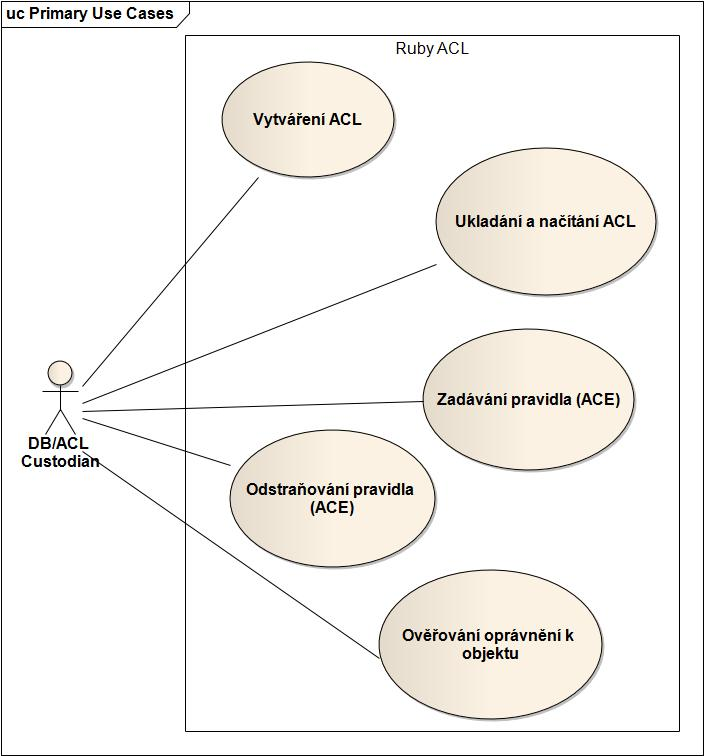
\includegraphics[width=15cm]{UseCases.jpg}
\caption{UseCases}
\label{fig:UseCases}
\end{figure}

%-------------------------------------

\subsection{Data flow diagram}
Data flow diagram (viz "Obrázek 2") znázorňuje tok dat mezi jednotlivými funkcemi aplikace. Popisuje funkce a jejich vazby. Uložiště pro ACL je používaná databáze. Pro každou databázi bude jedna instance Ruby-ACL.
\begin{figure}
%\centering
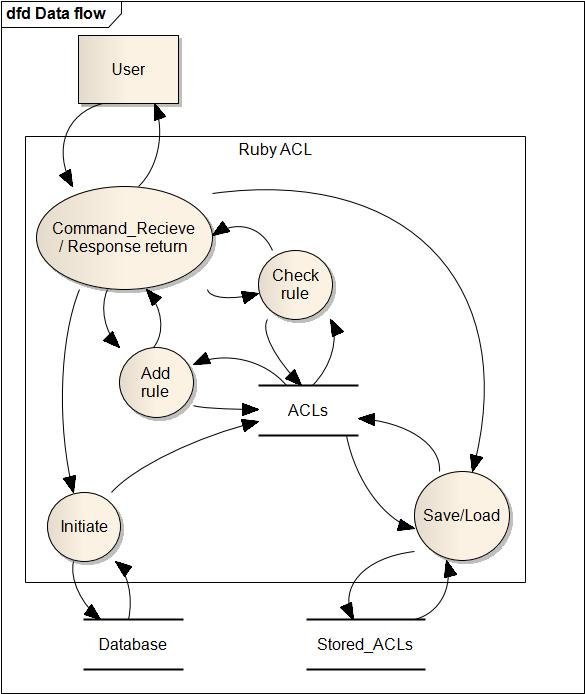
\includegraphics[width=15cm]{DataFlowBigFont.jpg}
\caption{Data flow diagram}
\label{fig:Data flow diagram}
\end{figure}

%-------------------------------------

\subsection{Class diagram}
Class diagram (viz "Obrázek 3") znázorňuje základní třídy aplikace a jejich vazby.
\begin{figure}
%\centering
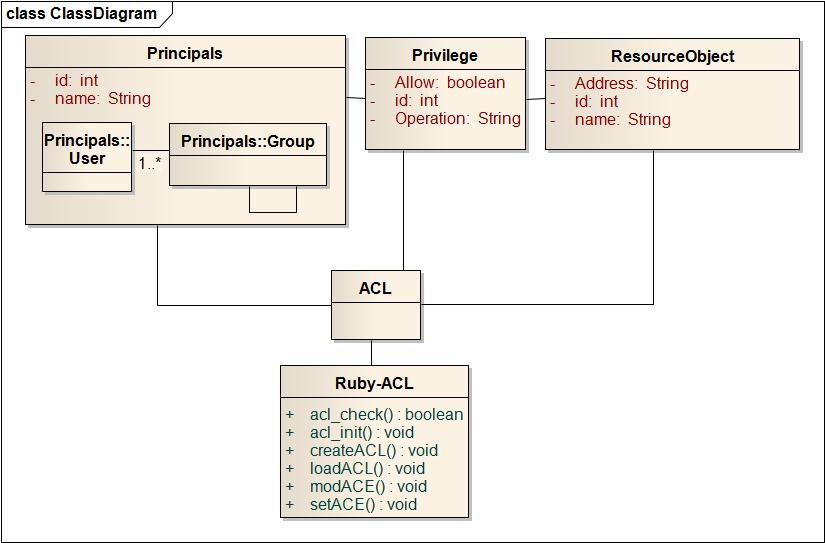
\includegraphics[width=15cm]{ClassDiagram2.jpg}
\caption{Class diagram}
\label{fig:Class diagram}
\end{figure}


%-------------------------------------
\newpage
\subsection{Oprávnění}
Ruby-ACL nabídne vlastní přidané privilegia a základní sadu privilegií a převzatých z Oracle potažmo MySQL. Jedná se o privilegia 'ALL PRIVILEGES', 'ALTER', 'CREATE', 'DELETE', 'DROP', 'FILE', 'INDEX', 'INSERT', 'PROCESS', 'REFERENCES', 'RELOAD', 'SELECT', 'SHUTDOWN', 'UPDATE' a 'USAGE'.

%*****************************************************************************
\chapter{Realizace}
Popis implementace/realizace se zaměřením na nestandardní části řešení.

\section{GIT}
%-------------------------------------
\section{Databáze}
Protože databáze Cellstore není plně funkční, nebylo možné implementaci testovat přímo na ní. Za tímto učelem se musela vybrat jiná podobná databáze.
\subsection{Sedna}


Sedna knihovna v Ruby poskytuje rozhraní pro databázi Sedna. Klient je Ruby rozšíření, které používá ovladač jazyka C, který je dodáván jako součást distribuce Sedna. To má být jednoduché a snadno použitelné. Ovšem zprovoznění knihovny Sedna neproběhlo tak hladce, jak se tvrdí.

\subsection{eXist-db}
eXist-db je open source systém pro správu databáze vytvořena pomocí technologie XML. Ukládá XML data podle datového modelu XML a nabízí efektivní a XQuery zpracování založené na indexování. Podporuje velké množství technologií. Uvedu zde pouze ty, které se týkají Ruby ACL: XPath 2.0(odkaz), XQuery(odkaz), XML-RPC(odkaz), XQuery Update Facility 1.0(odkaz)

XML databáze eXist-db se podobá Cellstore a byla doporučena vedoucím práce jako ideální. Přesto proběhly komplikace s XUpdate navzdory přesné interpretace dokumentace.

\subsubsection{komunikace}
Použití xQuery Update Facility místo xUpdate. (Možná vložím ukázku implementace)

\subsubsection{eXistDBAPI}
%-------------------------------------
\section{Pravidla rozhodování}
V této kapitole je popsáno jakým způsobem RubyACL rozhoduje o přidělení přístupu. 
Vše se odvijí od priority rozhodování

\subsection{Priorita rozhodování}

Nejnižší má největší prioritu.

\begin{enumerate}
\item Owner
\item Explicit Deny
\item Explicit Allow
\item Inherited Deny
\item Inherited Allow
\item If not found > Deny
\end{enumerate}

\subsubsection{Vlastník / Owner}
Owner může být jednotlivec, množina jednotlivců i skupina.
Množina jednotlivců je v případě pokud se od kořene zdrojových objektů k listu mnění vlastník. Vlastník nejnadřazenějšího zdroje má největší práva. Vlastník může být o 
/* nemá význam, protože vlastník zdrojového objektu vlastní i všechny podřazené zdrojové objekty.


%-------------------------------------
\section{Implementace}
\subsection{Uvolňování paměti}
Je třeba se věnovat uvolňování paměti, protože aplikace bude spuštěna dny až měsíce. Špatné zacházení s pamětí by, proto bylo kritické pro server, na kterém aplikace s Ruby-ACL knihovnou bude spuštěna.
\begin{itemize}
\item Ušetření času db serveru vhodným uspořádáním dotazů. Místo iterace dotazů jeden dotaz s vhodnou podmínkou. (tvoreni clenstvi) 
\item Pro identifikaci a propojení jsem uvažoval mezi xLink a idref. Idref nabízí jednoduchý systém, ale xLink nabídl podrobné specifikace W3C, velké množství návodů a turtoriálů a především se jedná o novější technologii, jejíž osvojení jsem považoval za výhodné. Rozhodl jsem se proto implementovat xLink. Problém nastal při některých vkládání textů a dotazování. EXist DB měla problém s jmeným prostorem xLink i přes zkutečnost, že jmený prostor byl uveden. Troufám si říct, že byl uveden správně, protože při většině použití fungoval. Než abych se zabýval mnoho času proč použití xLink nejde, raději jsem přešel na jednoduchý idref. Implementace idref proběhla bez problémů.
\item Občas je kód zdvojený, ale má to svoje opodstatnění. Například addmembership a addmembershippriv. Kdyby nebylo zdvojeno, šlo by přidávat privilige k principal a naopak.
\item predelavam structuru z tridniho volani na singleton nebo jak se to jmenuje.\item predelavam structuru z tridniho volani na singleton nebo jak se to jmenuje.
\item kdyz smazu nadrazenou skupinu tak smazu vsechny jeji clenstvi
\end{itemize}

%-------------------------------------

\begin{itemize}

\item id u resob. Pokud to bude poradi, mohlo byt snaze napadnutelne nez kdyby id nedavalo smysl.

\item eXist xpath chyba. Na dotaz 
\begin{verbatim}
doc("/db/test_acl/ResourceObjects.xml")/ResourceObjects/descendant::*[type="Rybnik"] najde 0 vysledky
\end{verbatim}
ale na dotaz 
\begin{verbatim}
doc("/db/test_acl/ResourceObjects.xml")/ResourceObjects/descendant::*[type="Rybnik"]/string(@id) najde 1 vysledek = "" (prazdny string)
\end{verbatim}

\item res\_ob se muzou vytvorit dopredu v seznamu res\_obs. Res\_ob musi byt kazdopadne v seznamu (vytvori se pri vytvoreni pravidla).

\item Use “all” or “*” to match any address.

\item vysledek rozhodnuti jde nechranenou cestou. pokud ma napadajici pristup ke kanalu mezi db a rubyacl potazmo db aplikaci, tak muze zmenit vysledek dotazu a tim i rozhodnuti.

\end{itemize}
%*****************************************************************************
\chapter{Testování}

\begin{itemize}
 \item Způsob, průběh a výsledky testování.
 \item Srovnání s existujícími řešeními, pokud jsou známy.
\end{itemize} 


%*****************************************************************************
\chapter{Závěr}

\begin{itemize}
\item Zhodnocení splnění cílů DP/BP a  vlastního přínosu práce (při formulaci je třeba vzít v potaz zadání práce).
\item Diskuse dalšího možného pokračování práce.
\end{itemize} 

%*****************************************************************************
% Seznam literatury je v samostatnem souboru reference.bib. Ten
% upravte dle vlastnich potreb, potom zpracujte (a do textu
% zapracujte) pomoci prikazu bibtex a nasledne pdflatex (nebo
% latex). Druhy z nich alespon 2x, aby se poresily odkazy.

% originally following specification for bibliography formating was used
%\bibliographystyle{abbrv}

% Here is an improvment by Petr Dlouhy (April 2010).
% It is mainly for supervisors who expect Czech fomrating rules for references
% Additional feature is live url addresses to sources from your pdf file
% It requires the file csplainnat.bst (included in this sample zipfile).

\bibliographystyle{csplainnat}

%bibliographystyle{plain}
%\bibliographystyle{psc}
{
%JZ: 11.12.2008 Kdo chce mit v techto ukazkovych odkazech take odkaz na CSTeX:
\def\CS{$\cal C\kern-0.1667em\lower.5ex\hbox{$\cal S$}\kern-0.075em $}
\bibliography{reference}
}

% M. Dušek radi:
%\bibliographystyle{alpha}
% kdy citace ma tvar [AutorRok] (napriklad [Cook97]). Sice to asi neni  podle ceske normy (BTW BibTeX stejne neodpovida ceske norme), ale je to nejprehlednejsi.
% 3.5.2009 JZ polemizuje: BibTeX neobvinujte, napiste a poskytnete nam styl (.bst) splnujici citacni normu CSN/ISO.

%*****************************************************************************
%*****************************************************************************
\appendix

\chapter{Testování zaplnění stránky a odsazení odstavců}
\textbf{\large Tato příloha nebude součástí vaší práce. 
Slouží pouze jako příklad formátování textu.}

\section*{}
Určitě existuje nějaká pěkná latinská věta, která se k tomuhle testování používá, ale co mají dělat ti, kteří se nikdy latinsky neučili? Určitě existuje nějaká pěkná latinská věta, která se k tomuhle testování používá, ale co mají dělat ti, kteří se nikdy latinsky neučili? Určitě existuje nějaká pěkná latinská věta, která se k tomuhle testování používá, ale co mají dělat ti, kteří se nikdy latinsky neučili?

Určitě existuje nějaká pěkná latinská věta, která se k tomuhle testování používá, ale co mají dělat ti, kteří se nikdy latinsky neučili? Určitě existuje nějaká pěkná latinská věta, která se k tomuhle testování používá, ale co mají dělat ti, kteří se nikdy latinsky neučili? Určitě existuje nějaká pěkná latinská věta, která se k tomuhle testování používá, ale co mají dělat ti, kteří se nikdy latinsky neučili?

Určitě existuje nějaká pěkná latinská věta, která se k tomuhle testování používá, ale co mají dělat ti, kteří se nikdy latinsky neučili? Určitě existuje nějaká pěkná latinská věta, která se k tomuhle testování používá, ale co mají dělat ti, kteří se nikdy latinsky neučili? Určitě existuje nějaká pěkná latinská věta, která se k tomuhle testování používá, ale co mají dělat ti, kteří se nikdy latinsky neučili?

Určitě existuje nějaká pěkná latinská věta, která se k tomuhle testování používá, ale co mají dělat ti, kteří se nikdy latinsky neučili? Určitě existuje nějaká pěkná latinská věta, která se k tomuhle testování používá, ale co mají dělat ti, kteří se nikdy latinsky neučili? Určitě existuje nějaká pěkná latinská věta, která se k tomuhle testování používá, ale co mají dělat ti, kteří se nikdy latinsky neučili? Určitě existuje nějaká pěkná latinská věta, která se k tomuhle testování používá, ale co mají dělat ti, kteří se nikdy latinsky neučili? Určitě existuje nějaká pěkná latinská věta, která se k tomuhle testování používá, ale co mají dělat ti, kteří se nikdy latinsky neučili? Určitě existuje nějaká pěkná latinská věta, která se k tomuhle testování používá, ale co mají dělat ti, kteří se nikdy latinsky neučili?

Určitě existuje nějaká pěkná latinská věta, která se k tomuhle testování používá, ale co mají dělat ti, kteří se nikdy latinsky neučili? Určitě existuje nějaká pěkná latinská věta, která se k tomuhle testování používá, ale co mají dělat ti, kteří se nikdy latinsky neučili?

Určitě existuje nějaká pěkná latinská věta, která se k tomuhle testování používá, ale co mají dělat ti, kteří se nikdy latinsky neučili? Určitě existuje nějaká pěkná latinská věta, která se k tomuhle testování používá, ale co mají dělat ti, kteří se nikdy latinsky neučili? Určitě existuje nějaká pěkná latinská věta, která se k tomuhle testování používá, ale co mají dělat ti, kteří se nikdy latinsky neučili? Určitě existuje nějaká pěkná latinská věta, která se k tomuhle testování používá, ale co mají dělat ti, kteří se nikdy latinsky neučili? Určitě existuje nějaká pěkná latinská věta, která se k tomuhle testování používá, ale co mají dělat ti, kteří se nikdy latinsky neučili?

Určitě existuje nějaká pěkná latinská věta, která se k tomuhle testování používá, ale co mají dělat ti, kteří se nikdy latinsky neučili? Určitě existuje nějaká pěkná latinská věta, která se k tomuhle testování používá, ale co mají dělat ti, kteří se nikdy latinsky neučili? Určitě existuje nějaká pěkná latinská věta, která se k tomuhle testování používá, ale co mají dělat ti, kteří se nikdy latinsky neučili? Určitě existuje nějaká pěkná latinská věta, která se k tomuhle testování používá, ale co mají dělat ti, kteří se nikdy latinsky neučili? Určitě existuje nějaká pěkná latinská věta, která se k tomuhle testování používá, ale co mají dělat ti, kteří se nikdy latinsky neučili?

Určitě existuje nějaká pěkná latinská věta, která se k tomuhle testování používá, ale co mají dělat ti, kteří se nikdy latinsky neučili? Určitě existuje nějaká pěkná latinská věta, která se k tomuhle testování používá, ale co mají dělat ti, kteří se nikdy latinsky neučili? Určitě existuje nějaká pěkná latinská věta, která se k tomuhle testování používá, ale co mají dělat ti, kteří se nikdy latinsky neučili? Určitě existuje nějaká pěkná latinská věta, která se k tomuhle testování používá, ale co mají dělat ti, kteří se nikdy latinsky neučili? Určitě existuje nějaká pěkná latinská věta, která se k tomuhle testování používá, ale co mají dělat ti, kteří se nikdy latinsky neučili?

Určitě existuje nějaká pěkná latinská věta, která se k tomuhle testování používá, ale co mají dělat ti, kteří se nikdy latinsky neučili? Určitě existuje nějaká pěkná latinská věta, která se k tomuhle testování používá, ale co mají dělat ti, kteří se nikdy latinsky neučili? Určitě existuje nějaká pěkná latinská věta, která se k tomuhle testování používá, ale co mají dělat ti, kteří se nikdy latinsky neučili? Určitě existuje nějaká pěkná latinská věta, která se k tomuhle testování používá, ale co mají dělat ti, kteří se nikdy latinsky neučili? Určitě existuje nějaká pěkná latinská věta, která se k tomuhle testování používá, ale co mají dělat ti, kteří se nikdy latinsky neučili?

Určitě existuje nějaká pěkná latinská věta, která se k tomuhle testování používá, ale co mají dělat ti, kteří se nikdy latinsky neučili? Určitě existuje nějaká pěkná latinská věta, která se k tomuhle testování používá, ale co mají dělat ti, kteří se nikdy latinsky neučili? Určitě existuje nějaká pěkná latinská věta, která se k tomuhle testování používá, ale co mají dělat ti, kteří se nikdy latinsky neučili? Určitě existuje nějaká pěkná latinská věta, která se k tomuhle testování používá, ale co mají dělat ti, kteří se nikdy latinsky neučili? Určitě existuje nějaká pěkná latinská věta, která se k tomuhle testování používá, ale co mají dělat ti, kteří se nikdy latinsky neučili?

Určitě existuje nějaká pěkná latinská věta, která se k tomuhle testování používá, ale co mají dělat ti, kteří se nikdy latinsky neučili? Určitě existuje nějaká pěkná latinská věta, která se k tomuhle testování používá, ale co mají dělat ti, kteří se nikdy latinsky neučili? Určitě existuje nějaká pěkná latinská věta, která se k tomuhle testování používá, ale co mají dělat ti, kteří se nikdy latinsky neučili? Určitě existuje nějaká pěkná latinská věta, která se k tomuhle testování používá, ale co mají dělat ti, kteří se nikdy latinsky neučili? Určitě existuje nějaká pěkná latinská věta, která se k tomuhle testování používá, ale co mají dělat ti, kteří se nikdy latinsky neučili?

Určitě existuje nějaká pěkná latinská věta, která se k tomuhle testování používá, ale co mají dělat ti, kteří se nikdy latinsky neučili? Určitě existuje nějaká pěkná latinská věta, která se k tomuhle testování používá, ale co mají dělat ti, kteří se nikdy latinsky neučili? Určitě existuje nějaká pěkná latinská věta, která se k tomuhle testování používá, ale co mají dělat ti, kteří se nikdy latinsky neučili? Určitě existuje nějaká pěkná latinská věta, která se k tomuhle testování používá, ale co mají dělat ti, kteří se nikdy latinsky neučili? Určitě existuje nějaká pěkná latinská věta, která se k tomuhle testování používá, ale co mají dělat ti, kteří se nikdy latinsky neučili?

Určitě existuje nějaká pěkná latinská věta, která se k tomuhle testování používá, ale co mají dělat ti, kteří se nikdy latinsky neučili? Určitě existuje nějaká pěkná latinská věta, která se k tomuhle testování používá, ale co mají dělat ti, kteří se nikdy latinsky neučili? Určitě existuje nějaká pěkná latinská věta, která se k tomuhle testování používá, ale co mají dělat ti, kteří se nikdy latinsky neučili? Určitě existuje nějaká pěkná latinská věta, která se k tomuhle testování používá, ale co mají dělat ti, kteří se nikdy latinsky neučili? Určitě existuje nějaká pěkná latinská věta, která se k tomuhle testování používá, ale co mají dělat ti, kteří se nikdy latinsky neučili?

Určitě existuje nějaká pěkná latinská věta, která se k tomuhle testování používá, ale co mají dělat ti, kteří se nikdy latinsky neučili? Určitě existuje nějaká pěkná latinská věta, která se k tomuhle testování používá, ale co mají dělat ti, kteří se nikdy latinsky neučili? Určitě existuje nějaká pěkná latinská věta, která se k tomuhle testování používá, ale co mají dělat ti, kteří se nikdy latinsky neučili? Určitě existuje nějaká pěkná latinská věta, která se k tomuhle testování používá, ale co mají dělat ti, kteří se nikdy latinsky neučili? Určitě existuje nějaká pěkná latinská věta, která se k tomuhle testování používá, ale co mají dělat ti, kteří se nikdy latinsky neučili?

Určitě existuje nějaká pěkná latinská věta, která se k tomuhle testování používá, ale co mají dělat ti, kteří se nikdy latinsky neučili? Určitě existuje nějaká pěkná latinská věta, která se k tomuhle testování používá, ale co mají dělat ti, kteří se nikdy latinsky neučili? Určitě existuje nějaká pěkná latinská věta, která se k tomuhle testování používá, ale co mají dělat ti, kteří se nikdy latinsky neučili? Určitě existuje nějaká pěkná latinská věta, která se k tomuhle testování používá, ale co mají dělat ti, kteří se nikdy latinsky neučili? Určitě existuje nějaká pěkná latinská věta, která se k tomuhle testování používá, ale co mají dělat ti, kteří se nikdy latinsky neučili?

Určitě existuje nějaká pěkná latinská věta, která se k tomuhle testování používá, ale co mají dělat ti, kteří se nikdy latinsky neučili? Určitě existuje nějaká pěkná latinská věta, která se k tomuhle testování používá, ale co mají dělat ti, kteří se nikdy latinsky neučili? Určitě existuje nějaká pěkná latinská věta, která se k tomuhle testování používá, ale co mají dělat ti, kteří se nikdy latinsky neučili? Určitě existuje nějaká pěkná latinská věta, která se k tomuhle testování používá, ale co mají dělat ti, kteří se nikdy latinsky neučili? Určitě existuje nějaká pěkná latinská věta, která se k tomuhle testování používá, ale co mají dělat ti, kteří se nikdy latinsky neučili?

Určitě existuje nějaká pěkná latinská věta, která se k tomuhle testování používá, ale co mají dělat ti, kteří se nikdy latinsky neučili? Určitě existuje nějaká pěkná latinská věta, která se k tomuhle testování používá, ale co mají dělat ti, kteří se nikdy latinsky neučili? Určitě existuje nějaká pěkná latinská věta, která se k tomuhle testování používá, ale co mají dělat ti, kteří se nikdy latinsky neučili? Určitě existuje nějaká pěkná latinská věta, která se k tomuhle testování používá, ale co mají dělat ti, kteří se nikdy latinsky neučili? Určitě existuje nějaká pěkná latinská věta, která se k tomuhle testování používá, ale co mají dělat ti, kteří se nikdy latinsky neučili?

Určitě existuje nějaká pěkná latinská věta, která se k tomuhle testování používá, ale co mají dělat ti, kteří se nikdy latinsky neučili? Určitě existuje nějaká pěkná latinská věta, která se k tomuhle testování používá, ale co mají dělat ti, kteří se nikdy latinsky neučili? Určitě existuje nějaká pěkná latinská věta, která se k tomuhle testování používá, ale co mají dělat ti, kteří se nikdy latinsky neučili? Určitě existuje nějaká pěkná latinská věta, která se k tomuhle testování používá, ale co mají dělat ti, kteří se nikdy latinsky neučili? Určitě existuje nějaká pěkná latinská věta, která se k tomuhle testování používá, ale co mají dělat ti, kteří se nikdy latinsky neučili?

Určitě existuje nějaká pěkná latinská věta, která se k tomuhle testování používá, ale co mají dělat ti, kteří se nikdy latinsky neučili? Určitě existuje nějaká pěkná latinská věta, která se k tomuhle testování používá, ale co mají dělat ti, kteří se nikdy latinsky neučili? Určitě existuje nějaká pěkná latinská věta, která se k tomuhle testování používá, ale co mají dělat ti, kteří se nikdy latinsky neučili? Určitě existuje nějaká pěkná latinská věta, která se k tomuhle testování používá, ale co mají dělat ti, kteří se nikdy latinsky neučili? Určitě existuje nějaká pěkná latinská věta, která se k tomuhle testování používá, ale co mají dělat ti, kteří se nikdy latinsky neučili?

Určitě existuje nějaká pěkná latinská věta, která se k tomuhle testování používá, ale co mají dělat ti, kteří se nikdy latinsky neučili? Určitě existuje nějaká pěkná latinská věta, která se k tomuhle testování používá, ale co mají dělat ti, kteří se nikdy latinsky neučili? Určitě existuje nějaká pěkná latinská věta, která se k tomuhle testování používá, ale co mají dělat ti, kteří se nikdy latinsky neučili? Určitě existuje nějaká pěkná latinská věta, která se k tomuhle testování používá, ale co mají dělat ti, kteří se nikdy latinsky neučili? Určitě existuje nějaká pěkná latinská věta, která se k tomuhle testování používá, ale co mají dělat ti, kteří se nikdy latinsky neučili?

%*****************************************************************************
\chapter{Pokyny a návody k formátování textu práce}
\textbf{\large Tato příloha samozřejmě nebude součástí vaší práce. Slouží pouze jako příklad formátování textu.}

Používat se dají všechny příkazy systému \LaTeX. Existuje velké množství volně přístupné dokumentace, tutoriálů, příruček a dalších materiálů v elektronické podobě. Výchozím bodem, kromě Googlu, může být stránka CSTUG (Czech Tech Users Group) \cite{CSTUG}. Tam najdete odkazy na další materiály.  Vetšinou dostačující a přehledně organizovanou elektronikou dokumentaci najdete například na \cite{latexdocweb} nebo \cite{latexwiki}.

Existují i různé nadstavby nad systémy \TeX{} a \LaTeX, které výrazně usnadní psaní textu zejména začátečníkům. Velmi rozšířený v Linuxovém prostředí je systém Kile.


\section{Vkládání obrázků}
Obrázky se umísťují do plovoucího prostředí \verb|figure|. Každý obrázek by měl obsahovat \textbf{název} (\verb|\caption|) a \textbf{návěští} (\verb|\label|). Použití příkazu pro vložení obrázku \\\verb|\includegraphics| je podmíněno aktivací (načtením) balíku graphicx příkazem\\ \verb|\usepackage{graphicx}|.

Budete-li zdrojový text zpracovávat pomocí programu \verb|pdflatex|, očekávají se obrázky s příponou \verb|*.pdf|\footnote{pdflatex umí také formáty PNG a JPG.}, použijete-li k formátování \verb|latex|, očekávají se obrázky s příponou \verb|*.eps|.\footnote{Vzájemnou konverzi mezi snad všemi typy obrazku včetně změn vekostí a dalších vymožeností vám může zajistit balík ImageMagic  (http://www.imagemagick.org/script/index.php). Je dostupný pod Linuxem, Mac OS i MS Windows. Důležité jsou zejména příkazy convert a identify.}

\begin{figure}[ht]
\begin{center}

\includegraphics[width=5cm]{figures/LogoCVUT}
\caption{Popiska obrázku}
\label{fig:logo}
\end{center}
\end{figure}

Příklad vložení obrázku:
\begin{verbatim}
\begin{figure}[h]
\begin{center}

\includegraphics[width=5cm]{figures/LogoCVUT}
\caption{Popiska obrazku}
\label{fig:logo}
\end{center}
\end{figure}
\end{verbatim}

\section{Kreslení obrázků}
Zřejmě každý z vás má nějaký oblíbený nástroj pro tvorbu obrázků. Jde jen o to, abyste dokázali obrázek uložit v požadovaném formátu nebo jej do něj konvertovat (viz předchozí kapitola). Je zřejmě vhodné kreslit obrázky vektorově. Celkem oblíbený, na ovládání celkem jednoduchý a přitom dostatečně mocný je například program Inkscape.

Zde stojí za to upozornit na kreslící programe Ipe \cite{ipe}, který dokáže do obrázku vkládat komentáře přímo v latexovském formátu (vzroce, stejné fonty atd.). Podobné věci umí na Linuxové platformě nástroj Xfig. 

Za pozornost ještě stojí schopnost editoru Ipe importovat obrázek (jpg nebo bitmap) a krelit do něj latexovské popisky a komentáře. Výsledek pak umí exportovat přímo do pdf.

\section{Tabulky}
Existuje více způsobů, jak sázet tabulky. Například je možno použít prostředí \verb|table|, které je velmi podobné prostředí \verb|figure|. 

\begin{table}
\begin{center}
\begin{tabular}{|c|l|l|}
\hline
\textbf{DTD} & \textbf{construction} & \textbf{elimination} \\
\hline
$\mid$ & \verb+in1|A|B a:sum A B+ & \verb+case([_:A]a)([_:B]a)ab:A+\\
&\verb+in1|A|B b:sum A B+ & \verb+case([_:A]b)([_:B]b)ba:B+\\
\hline
$+$&\verb+do_reg:A -> reg A+&\verb+undo_reg:reg A -> A+\\
\hline
$*,?$& the same like $\mid$ and $+$ & the same like $\mid$ and $+$\\
& with \verb+emtpy_el:empty+ & with \verb+emtpy_el:empty+\\
\hline
R(a,b) & \verb+make_R:A->B->R+ & \verb+a: R -> A+\\
 & & \verb+b: R -> B+\\
\hline
\end{tabular}
\end{center}
\caption{Ukázka tabulky}
\label{tab:tab1}
\end{table}

Zdrojový text tabulky \ref{tab:tab1} vypadá takto:
\begin{verbatim}
\begin{table}
\begin{center}
\begin{tabular}{|c|l|l|}
\hline
\textbf{DTD} & \textbf{construction} & \textbf{elimination} \\
\hline
$\mid$ & \verb+in1|A|B a:sum A B+ & \verb+case([_:A]a)([_:B]a)ab:A+\\
&\verb+in1|A|B b:sum A B+ & \verb+case([_:A]b)([_:B]b)ba:B+\\
\hline
$+$&\verb+do_reg:A -> reg A+&\verb+undo_reg:reg A -> A+\\
\hline
$*,?$& the same like $\mid$ and $+$ & the same like $\mid$ and $+$\\
& with \verb+emtpy_el:empty+ & with \verb+emtpy_el:empty+\\
\hline
R(a,b) & \verb+make_R:A->B->R+ & \verb+a: R -> A+\\
 & & \verb+b: R -> B+\\
\hline
\end{tabular}
\end{center}
\caption{Ukázka tabulky}
\label{tab:tab1}
\end{table}
\begin{table}
\end{verbatim}

\section{Odkazy v textu}
\subsection{Odkazy na literaturu}
Jsou realizovány příkazem \verb|\cite{odkaz}|. 

Seznam literatury je dobré zapsat do samostatného souboru a ten pak zpracovat programem bibtex (viz soubor \verb|reference.bib|). Zdrojový soubor pro \verb|bibtex| vypadá například takto:
\begin{verbatim}
@Article{Chen01,
  author  = "Yong-Sheng Chen and Yi-Ping Hung and Chiou-Shann Fuh",
  title   = "Fast Block Matching Algorithm Based on 
             the Winner-Update Strategy",
  journal = "IEEE Transactions On Image Processing",
  pages   = "1212--1222",
  volume  =  10,
  number  =   8,
  year    = 2001,
}

@Misc{latexdocweb,
  author  = "",
  title   = "{\LaTeX} --- online manuál",
  note    = "\verb|http://www.cstug.cz/latex/lm/frames.html|",
  year    = "",
}
...
\end{verbatim}

%11.12.2008, 3.5.2009
\textbf{Pozor:} Sazba názvů odkazů je dána Bib\TeX{} stylem\\ (\verb|\bibliographystyle{abbrv}|). 
%Budete-li používat české prostředí (\verb|\usepackage[czech]{babel}|), 
Bib\TeX{} tedy obvykle vysází velké pouze počáteční písmeno z názvu zdroje, 
ostatní písmena zůstanou malá bez ohledu na to, jak je napíšete. 
Přesněji řečeno, styl může zvolit pro každý typ publikace jiné konverze. 
Pro časopisecké články třeba výše uvedené, jiné pro monografie (u nich často bývá 
naopak velikost písmen zachována).

Pokud chcete Bib\TeX u napovědět, která písmena nechat bez konverzí 
(viz \texttt{title = "\{$\backslash$LaTeX\} -{}-{}- online manuál"} 
v~předchozím příkladu), je nutné příslušné písmeno (zde celé makro) uzavřít 
do složených závorek. Pro přehlednost je proto vhodné celé parametry 
uzavírat do uvozovek (\texttt{author = "\dots"}), nikoliv do složených závorek.

Odkazy na literaturu ve zdrojovém textu se pak zapisují:
\begin{verbatim}
Podívejte se na \cite{Chen01}, 
další detaily najdete na \cite{latexdocweb}
\end{verbatim}

Vazbu mezi soubory \verb|*.tex| a \verb|*.bib| zajistíte příkazem 
\verb|\bibliography{}| v souboru \verb|*.tex|.  V našem případě tedy zdrojový 
dokument \verb|thesis.tex| obsahuje příkaz\\
\verb|\bibliography{reference}|.

Zpracování zdrojového textu s odkazy se provede postupným voláním programů\\
\verb|pdflatex <soubor>| (případně \verb|latex <soubor>|), \verb|bibtex <soubor>| 
a opět\\ \verb|pdflatex <soubor>|.\footnote{První volání \texttt{pdflatex} 
vytvoří soubor s~koncovkou \texttt{*.aux}, který je vstupem pro program 
\texttt{bibtex}, pak je potřeba znovu zavolat program \texttt{pdflatex} 
(\texttt{latex}), který tentokrát zpracuje soubory s příponami \texttt{.aux} a 
\texttt{.tex}. 
Informaci o případných nevyřešených odkazech (cross-reference) vidíte přímo při 
zpracovávání zdrojového souboru příkazem \texttt{pdflatex}. Program \texttt{pdflatex} 
(\texttt{latex}) lze volat vícekrát, pokud stále vidíte nevyřešené závislosti.}


Níže uvedený příklad je převzat z dříve existujících pokynů studentům, kteří 
dělají svou diplomovou nebo bakalářskou práci v~Grafické skupině.\footnote{Několikrát 
jsem byl upozorněn, že web s těmito pokyny byl zrušen, proto jej zde přímo necituji. 
Nicméně příklad sám o sobě dokumentuje obecně přijímaný konsensus ohledně citací 
v~bakalářských a diplomových pracích na KP.} Zde se praví:
\begin{small}
\begin{verbatim}
...
j) Seznam literatury a dalších použitých pramenů, odkazy na WWW stránky, ...
 Pozor na to, že na veškeré uvedené prameny se musíte v textu práce 
 odkazovat -- [1]. 
Pramen, na který neodkazujete, vypadá, že jste ho vlastně nepotřebovali 
a je uveden jen do počtu. Příklad citace knihy [1], článku v časopise [2], 
stati ve sborníku [3] a html odkazu [4]: 
[1] J. Žára, B. Beneš;, and P. Felkel. 
     Moderní počítačová grafika. Computer Press s.r.o, Brno, 1 edition, 1998. 
     (in Czech). 
[2] P. Slavík. Grammars and Rewriting Systems as Models for Graphical User 
     Interfaces. Cognitive Systems, 4(4--3):381--399, 1997. 
[3] M. Haindl, Š. Kment, and P. Slavík. Virtual Information Systems. 
     In WSCG'2000 -- Short communication papers, pages 22--27, Pilsen, 2000. 
     University of West Bohemia. 
[4] Knihovna grafické skupiny katedry počítačů: 
     http://www.cgg.cvut.cz/Bib/library/ 
\end{verbatim}
\end{small}
\ldots{} abychom výše citované odkazy skutečně našli v (automaticky generovaném) seznamu literatury tohoto textu, musíme je nyní alespoň jednou citovat: Kniha \cite{kniha}, článek v~časopisu \cite{clanek}, příspěvek na konferenci \cite{sbornik}, www odkaz \cite{www}.

Ještě přidáme další ukázku citací online zdrojů podle české normy. Odkaz na wiki o frameworcich \cite{wiki:framework} a ORM \cite{wiki:orm}. Použití viz soubor \verb|reference.bib|. V seznamu literatury by nyní měly být živé odkazy na zdroje. V \verb|reference.bib| je zcela nový typ publikace. Detaily dohledal a dodal Petr Dlouhý v dubnu 2010. Podrobnosti najdete ve zdrojovém souboru tohoto textu v komentáři u příkazu \verb|\thebibliography|.

\subsection{Odkazy na obrázky, tabulky a kapitoly}
\begin{itemize}
\item Označení místa v textu, na které chcete později čtenáře práce odkázat, se provede příkazem \verb|\label{navesti}|. Lze použít v prostředích \verb|figure| a  \verb|table|, ale též za názvem kapitoly nebo podkapitoly.
\item Na návěští se odkážeme příkazem \verb|\ref{navesti}| nebo \verb|\pageref{navesti}|.
\end{itemize}

\section{Rovnice, centrovaná, číslovaná matematika}
Jednoduchý matematický výraz zapsaný přímo do textu se vysází pomocí prostředí \verb|math|, resp. zkrácený zápis pomocí uzavření textu rovnice mezi znaky \verb|$|.

Kód \verb|$ S = \pi * r^2 $| bude vysázen takto: $ S = \pi * r^2 $.

Pokud chcete nečíslované rovnice, ale umístěné centrovaně na samostatné řádky, pak lze použít prostředí \verb|displaymath|, resp. zkrácený zápis pomocí uzavření textu rovnice mezi znaky \verb|$$|. Zdrojový kód: 
\begin{verb}
|$$ S = \pi * r^2 $$|
\end{verb}
bude pak vysázen takto:
$$ S = \pi * r^2 $$

Chcete-li mít rovnice číslované, je třeba použít prostředí \verb|eqation|. Kód:
\begin{verbatim}
\begin{equation}
  S = \pi * r^2
\end{equation}

\begin{equation}
  V = \pi * r^3
\end{equation}
\end{verbatim}
je potom vysázen takto:
\begin{equation}
  S = \pi * r^2
\end{equation}

\begin{equation}
  V = \pi * r^3
\end{equation}

\section{Kódy programu}
Chceme-li vysázet například část zdrojového kódu programu (bez formátování), hodí se prostředí \verb|verbatim|: 
\begin{verbatim}
         (* nickname2 *)
Lego> Refine in1
             (do_reg (nickname1 h));
Refine by  in1 (do_reg (nickname1 h))
   ?4 : pcdata
   ?5 : pcdata
          (* surname2 *)
Lego> Refine surname1 h;
Refine by  surname1 h
   ?5 : pcdata
          (* email2 *)
Lego> Refine undo_reg (email1 h);
Refine by  undo_reg (email1 h)
*** QED ***
\end{verbatim}

\section{Další poznámky}
\subsection{České uvozovky}
V souboru \verb|k336_thesis_macros.tex| je příkaz \verb|\uv{}| pro sázení českých uvozovek. \uv{Text uzavřený do českých uvozovek.}

% JZ: 3.5.2009 \chapter z book zajistí automaticky
%\subsection{Začátky kapitol na liché stránky}
%Ve výsledném textu je dobré, když každá kapitola začíná na liché stránce. Tedy použijte:
%\begin{verbatim}
%  \cleardoublepage\chapter{Úvod}

\section{Úvod do problematiky}

Tato bakalářská práce navazuje na můj semestrální projekt. Zabývá se správou - administrací řízení přístupu, jakožto procesu autorizování uživatelů, skupin a počítačů pro přístup k objektům. Tento proces pracuje s pojmy: oprávnění, uživatelská práva a audit objektů. Tato jednotlivá přiřazená oprávnění začleňuje jako položky řízení přístupu (ACE\footnote{Access Control Entry}) a jejich celé sady začleňuje do seznamu přístupových práv (ACL\footnote{Access Control List}). Úkolem bakalářské práce bylo vytvořit, navrhnout a realizovat v jazyce Ruby model uživatelských přístupových práv určený pro objektovou XML\footnote{Extensible Markup Language} databázi.

Součástí práce byl návrh knihovny. Navržená knihovna realizuje správu řízení přístupu pomocí ACL. Knihovnu nazývám Ruby-ACL. Protože moje bakalářská práce je prací implementační, včetně testů navržené knihovny, zaměřil jsem se na specifikaci rozhraní knihovny a na příklady jejího použití. Výsledkem je nejen samotná realizace knihovny, ale i podrobná programátorská dokumentace.

Je-li potřeba zabezpečit zdroje a jeho prostředky, je nutné vzít v úvahu, jakými právy budou disponovat ti, kteří k nim budou přistupovat. Zabezpečit objekt, například dokument či kolekci, lze přidělením oprávnění, která umožňují uživatelům nebo skupinám provádět u tohoto objektu určité akce. Řízení přístupů je činnost zabývající se přidáváním a zamítáním oprávnění přistupujícím.

Ruby je objektově orientovaný, interpretovaný skriptovací programovací jazyk. Díky své jednoduché syntaxi je poměrně snadný, přesto však dostatečně výkonný, aby dokázal konkurovat známějším jazykům jako je Python a Perl. Převzato a upraveno z wikipedie\cite{wiki:Ruby}

ACL je seznam pro řízení přístupů. Seznam určuje, kdo nebo co má povolení přistupovat k objektu a jaké operace s ním může nebo nesmí provádět. V typickém ACL specifikuje každý záznam v seznamu uživatele a operaci\cite{wiki:acl}.

%-------------------------------

\section{Motivace}
Zaujala mě problematika práv, databází a pro mě neznámého jazyka Ruby.
Jádro celé mé motivace, bylo projít si vývojem softwaru, v tomto případě knihovny, od návrhu přes implementaci k testování a dokumentaci a ověřit si získané poznatky z předmětu softwarového inženýrství. Soustředil jsem se na vlastní nápady. Nechtěl jsem skládat a kopírovat polotvary a "lepit" je dohromady.
%  \cleardoublepage\include{2_teorie}
%   atd.\ldots{}
%\end{verbatim}

%*****************************************************************************
\chapter{Seznam použitých zkratek}

\begin{description}
\item[2D] Two-Dimensional
\item[ABN] Abstract Boolean Networks
\item[ASIC] Application-Specific Integrated Circuit
\end{description}
\vdots

%*****************************************************************************
\chapter{UML diagramy}
\textbf{\large Tato příloha není povinná a zřejmě se neobjeví v každé práci. Máte-li ale větší množství podobných diagramů popisujících systém, není nutné všechny umísťovat do hlavního textu, zvláště pokud by to snižovalo jeho čitelnost.}

%*****************************************************************************
\chapter{Instalační a uživatelská příručka}
\textbf{\large Tato příloha velmi žádoucí zejména u softwarových implementačních prací.}

%*****************************************************************************
\chapter{Obsah přiloženého CD}
\textbf{\large Tato příloha je povinná pro každou práci. Každá práce musí totiž obsahovat přiložené CD. Viz dále.}

Může vypadat například takto. Váš seznam samozřejmě bude odpovídat typu vaší práce. (viz \cite{infodp}):

\begin{figure}[h]
\begin{center}
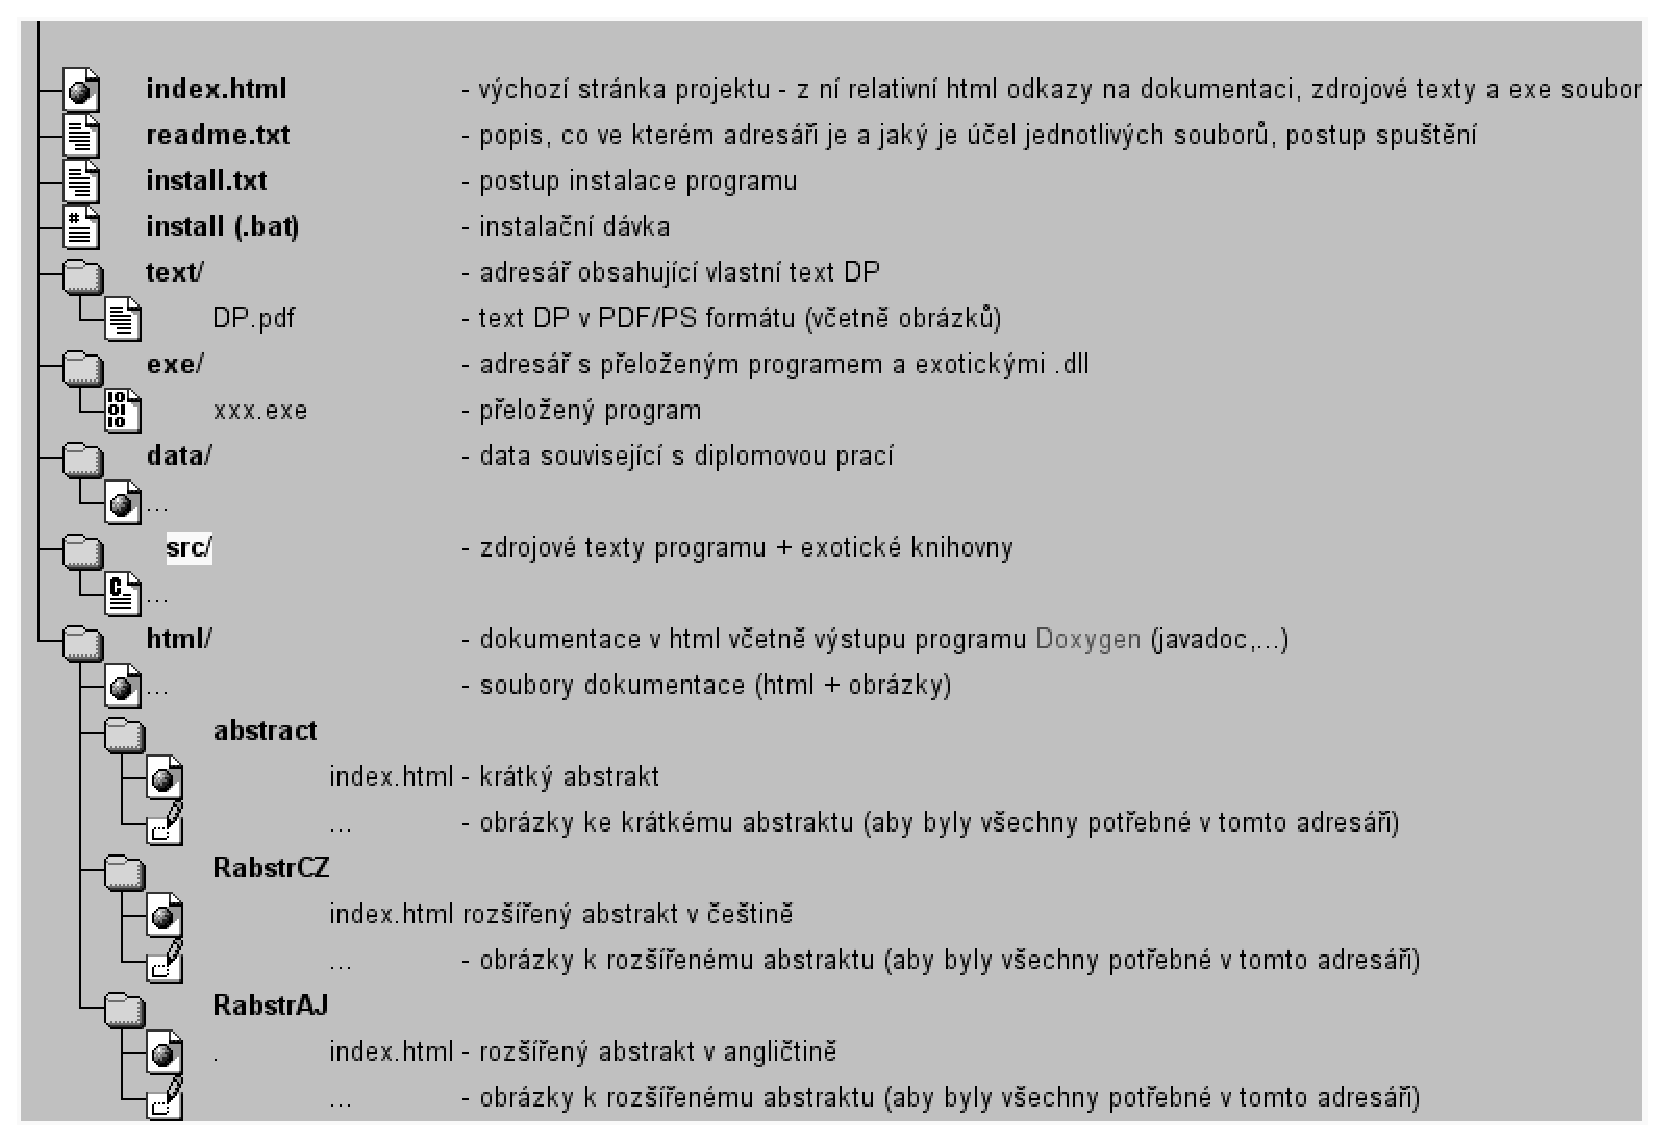
\includegraphics[width=14cm]{figures/seznamcd}
\caption{Seznam přiloženého CD --- příklad}
\label{fig:seznamcd}
\end{center}
\end{figure}

Na GNU/Linuxu si strukturu přiloženého CD můžete snadno vyrobit příkazem:\\ 
\verb|$ tree . >tree.txt|\\
Ve vzniklém souboru pak stačí pouze doplnit komentáře.

Z \textbf{README.TXT} (případne index.html apod.)  musí být rovněž zřejmé, jak programy instalovat, spouštět a jaké požadavky mají tyto programy na hardware.

Adresář \textbf{text}  musí obsahovat soubor s vlastním textem práce v PDF nebo PS formátu, který bude později použit pro prezentaci diplomové práce na WWW.

\end{document}
